% This template was originally by R. Jacob Vogelstein
% Updated on March 1, 2010 by Noah J. Cowan
% Updated on May 18, 2014 by Brian Weitzner
% at https://github.com/weitzner/jhu-thesis-template
% Updated on January 29, 2016 by John Muschelli
% at https://github.com/muschellij2/PhD_Thesis
% Updated on April 13, 2016 by Leonardo Collado Torres and
% available at https://github.com/lcolladotor/jhu-thesis-template.
% Forked by John Clayton in December, 2019
% JHU Formatting requirements of Sheridan Libraries may be found at:
% https://www.library.jhu.edu/library-services/
% electronic-theses-dissertations/formatting-requirements/

% The document is based on the standard 12pt LaTeX report class
%\documentclass[12pt,draft]{report}
\documentclass[12pt]{report}

% PDF Creation settings
\pdfcompresslevel=9
\pdfminorversion=5
\pdfobjcompresslevel=2

% Needed to create a PDF/A file
\usepackage[a-1b]{pdfx}

% Incude pdf docs
\usepackage{pdfpages}
% For transferring hyperlinks from PDFs added by pdfpages
\usepackage{pax}

% For dialect-specific hyphenation etc.
\usepackage[american]{babel}

% T1 font encoding
\usepackage[T1]{fontenc}
% Use UTF8 input encoding
\usepackage[utf8]{inputenc}
%\DeclareUnicodeCharacter{00A0}{ }

% Load latin modern, a font with all the characters
\usepackage{lmodern}

% For generating the dummy text in the mwe template
\usepackage{lipsum}

% Provides various text symbols (such as \textdegree) in TS1 encoding.
\usepackage{textcomp}

% provides ul for cv
\usepackage{soul}

% Set the margins according to JHU specifications
\usepackage{geometry}
 \geometry{
   letterpaper,
   left=1.5in,
   right=1.0in,
   top=1.0in,
   bottom=1.0in}

% Spacing options
\usepackage{setspace}

% Typography and fonts
\usepackage[protrusion]{microtype}
% For multiple columns
\usepackage{multicol}
% for proper text wrapping of nucleic acid sequences
\usepackage{seqsplit}

% Fancy verbatim-like environment for code
\usepackage{listings}
\lstset{basicstyle=\footnotesize\ttfamily,
        columns=flexible,
        breaklines=true
}

% Hyperlink handling
\usepackage[pdfa]{hyperref}
\hypersetup{
   linktocpage,
   unicode,
   colorlinks=true,
   citecolor=link,
   filecolor=link,
   linkcolor=link,
   urlcolor=link
}

% Color handling
\usepackage{xcolor}
%\usepackage{color}

% Color for links
\definecolor{link}{rgb}{0.45,0.51,0.67}

%%% Table of Contents %%%
\usepackage[titles]{tocloft}
% Dots for chapters too
\renewcommand{\cftchapleader}{\cftdotfill{\cftdotsep}}

% To add bibliography to the table of contents
\usepackage{tocbibind}

% Set depth of TOC items
\setcounter{tocdepth}{4}

% Set depth of section numbering
\setcounter{secnumdepth}{4}

\usepackage{calc}
% Tweak to TOC to add 'chapter' to chapter name instead of a number only
\renewcommand{\cftchappresnum}{\chaptername\space}
% Set width of box based on longest label name
\setlength{\cftchapnumwidth}{\widthof{\textbf{Appendix~II~}}}

% Stylize chapter headings
%\usepackage{sectsty}
%\chapterfont{\centering}

% Removes 'Chapter #' title while keeping
% it listed in the TOC
\newcommand\chap[1]{%
  \chapter*{#1}%
  \addcontentsline{toc}{chapter}{#1}}

% Removes 'Section #' title while keeping
% it listed in the TOC
\newcommand\sect[1]{%
  \section*{#1}%
  \addcontentsline{toc}{section}{#1}}

% Removes 'Subsection #'title while keeping
% it listed in the TOC
\newcommand\subsect[1]{%
  \subsection*{#1}%
  \addcontentsline{toc}{subsection}{#1}}

% For oligo table
% Changes dot to hyphen in figure references and captions
\renewcommand{\thetable}{\thechapter-\Roman{table}}
\usepackage{booktabs}
\usepackage{multirow}
\usepackage{longtable}
\usepackage{array}
\usepackage{pdflscape}

% Align on numeric decimal in table
%\usepackage{dcolumn}

% Enhanced control over layout of itemize, enumerate, and description
\usepackage{enumitem}

% Graphics Packages
%\usepackage{graphics} 
\usepackage{graphicx}
%\usepackage{float}

% Setup style for figure captions
\usepackage[font=small,
            labelfont=bf,
            labelsep=period,
            font=sf,
            hypcap=true]{caption}

% For captions on the side of figures
\usepackage{ifthen}
\usepackage[rightcaption]{sidecap}

% Individual panel captions
%\usepackage{subfig}

% Options for hyperlinking to floats
\usepackage[all]{hypcap}

% Graphics Path
\graphicspath{{../images/}}

% To change the name of the figures page
\renewcommand{\listfigurename}{Figures}
% To change the default beginning to each line
\renewcommand{\cftfigpresnum}{\bfseries Figure }
% Changes dot to hyphen in figure references and captions
\renewcommand{\thefigure}{\thechapter-\arabic{figure}}
% To change the distance to the start of the figure title
\setlength{\cftfignumwidth}{\widthof{\textbf{Figure~5-10~}}}

% Tikz, for drawing vector graphics
%\usepackage{tikz}
%\usetikzlibrary{positioning}
%\usetikzlibrary{shapes,arrows}

% Enable the glossary
%\makeglossary

% Make appendices
%\usepackage[title,titletoc]{appendix}
\usepackage{appendix}
%\renewcommand{\appendixname}{Appendix}

%%%%%%%%%%%%%%%%%%
% FOR BIBTEX
%%%%%%%%%%%%%%%%%%

% For use with IEEEtran.bst
%\usepackage{cite}
%\usepackage[numbers,square,compress]{natbib}
%\setlength\bibsep{4pt}
% Set bibliography name
%\usepackage{chbibref}
%\renewcommand\bibname{References}

%%%%%%%%%%%%%%%%%%
% FOR BIBLATEX
%%%%%%%%%%%%%%%%%%

\usepackage[
style = nature, 
sorting = none, 
%dashed = false,
%maxbibnames = 99,
backend = biber,
url=false,
isbn=false,
natbib = true
]{biblatex}

% Point to bibfile
\addbibresource{bibtex.bib}

% If you want to exclude some portions from the bibliography
%\AtEveryBibitem{
%\clearfield{issn}
%\clearfield{note}
%\clearfield{month}
%}

% Change bib font size
\renewcommand{\bibfont}{\small}

%%%%%%%%%%%%%%%%%%
% DOI from Segmentation (needs hyperref)
%%%%%%%%%%%%%%%%%%

%\makeatletter
%\providecommand{\doi}[1]{%
%  \begingroup
%    \let\bibinfo\@secondoftwo
%    \urlstyle{rm}%
%    \href{http://dx.doi.org/#1}{%
%      doi:\discretionary{}{}{}%
%      \nolinkurl{#1}%
%    }%
%  \endgroup
%}
%\makeatother

% Math
%\usepackage{amsmath,amssymb,array}

%\newcommand{\bm}[1]{ \mbox{\boldmath $ #1 $} }
%\newcommand{\bin}[2]{\left(\begin{array}{@{}c@{}} #1 \\ #2
%             \end{array}\right) }
% A math shortcut frequently used by John Muschelli
%\newcommand{\bbeta}{\mbox{\boldmath $\beta$}}

%%%%%%%%%%%
% CONTENT %
%%%%%%%%%%%
%
\begin{document}
% Sets paragraph (and not title) spacing, roughly speaking
\setlength{\parskip}{3pt}
\baselineskip=24pt
%
% front matter page numbering
\pagenumbering{roman}
%
% Add title page
% JHU Dissertation title page
\thispagestyle{empty}
% baselineskip of 18pts (i.e. 1.5x spacing or 0.25")
% with 12pt type; 72 points per inch
\baselineskip=18pt
\begin{center}
% Spacer at top of page
\vspace*{3\baselineskip}
%
% TITLE GOES HERE
{\bfseries Malicious Network Traffic Detection via Deep Learning: \\An Information Theoretic View}\\[6\baselineskip]
%
by\\
%
% AUTHOR GOES HERE
Erick Galinkin\\[3\baselineskip]
%
%
A thesis submitted to The Johns Hopkins University in conformity\\
with the requirements for the degree of \\
Master of Science in Applied and Computational Mathematics\\[4\baselineskip]
%
Baltimore, Maryland\\
% DATE OF SUBMISSION HERE
June, 2020\\[6\baselineskip]
%
% UPDATE THE YEAR HERE
{\copyright{} 2020 E.~Galinkin\\
All rights reserved}
%
\end{center}
%
% Reset baseline skip to previous value
\baselineskip=24pt
\newpage 

%
% Setup and add front matter
\pagestyle{plain}
\setcounter{page}{2}
%
% Add abstract
\chapter*{Abstract}
%
The attention that deep learning has garnered from the academic community and industry continues to grow year over year, and it has been said that we are in a new golden age of artificial intelligence research.
However, neural networks are still often seen as a ``black box'' where learning occurs but cannot be understood in a formal way.
Using information geometry, we explore how homeomorphism affects the manifold on which learning occurs and the invariance of the mutual information captured by the coordinate system on that manifold under homeomorphism.
We empirically validate these results, using accuracy as a measure of similarity of learned representations.

Our results suggest that although the details of learned representations and the specific coordinate system defined over the manifold of all parameters differ slightly, the functional approximations are the same.
Furthermore, our results show that since mutual information remains invariant under homeomorphism, only feature engineering methods which alter the entropy of the dataset will change the outcome of the neural network.
Additionally, we show that for some datasets and tasks, neural networks require meaningful, human-driven feature engineering or changes in architecture to provide enough information for the neural network to generate a sufficient statistic.
Applying our results can serve to guide analysis methods for machine learning engineers and suggests that neural networks which can exploit the convolution theorem are equally accurate as standard convolutional neural networks, and can be more computationally efficient.
%
% Add Thesis Readers
\section*{Thesis Readers}
\begin{singlespace}
%
\noindent Dr.~Cleon Davis (Primary Advisor)\\
\indent \indent Senior Professional Staff\\
\indent \indent Johns Hopkins University Applied Physics Laboratory\\

\indent \indent and\\

\indent \indent Program Vice Chair Electrical and Computer Engineering\\
\indent \indent Lecturer and Research Faculty in Applied and Computational Mathematics\\
\indent \indent Johns Hopkins Engineering for Professionals\\


\noindent Dr.~Lanier Watkins\\
\indent \indent Program Chair\\
\indent \indent Department of Computer Science and Cybersecurity\\
\indent \indent Johns Hopkins University\\
\end{singlespace}
%
% Add readers (JHU style is to include readers with in abstract)
%\include{text/03-committee}
%
% Add preface
%\include{text/04-preface}
%
% Add dedication
% Adds a spacer where the header would be
\chapter*{~}
\addcontentsline{toc}{chapter}{Dedication}

\begin{center}
Y'all ain't ready - fuckin haters.
\end{center}

%
% Add acknowledgements
\chap{Acknowledgements}
%\addcontentsline{toc}{chapter}{Acknowledgements}

% INSERT TEXT HERE
I would like to extend my deepest gratitude to my thesis adviser, Cleon Davis, and my co-adviser Lanier Watkins.
I have learned so much in this process and you both have been incredibly supportive. 
No matter how far out over my skis I got, they found a way to pull me back in.
I hope that in the future, I will make you both proud to call me a peer.

I would also like to extend my gratitude to both Dr. Raymond Canzanese of Netskope, who was my work supervisor during much of my time at Johns Hopkins and Mr. Derek Abdine, who is my current work supervisor and was my supervisor during the writing of this thesis.
You have both always been patient, understanding, and flexible.
Without the two of you, I would likely not be continuing on in academia after this thesis, and I will forever be in your debt.

I would like to extend my gratitude to my colleague and friend Stella Biderman for all the time she spent hearing my crazy ideas and helping me contextualize them.

Lastly, my thanks to my dearest friends Dave and Emilee; the entire Rupeethon crew (Jon, Rich, Conor, Lynn, Scott, Steve); and my friends in the DEF CON AI village (Ariel, Rich, Sven, Yaga). 
No matter how galaxy-brained I got, you always listened and kept me inspired.
%
% To change the name of the contents page
%\renewcommand{\contentsname}{Contents}
%
% Create table of contents
\tableofcontents
%
% Create table list
%\listoftables
%
% Create List of figures
\listoffigures
\clearpage
%
%%% END FRONT MATTER %%%
%
%%%%% MAIN MATTER %%%%%
% Switch page numbering at the end of front matter, before first chapter
\pagenumbering{arabic}
%
%\begin{refsection}[myrefs.bib]
\chapter{Introduction}
\label{chap:intro}

\sect{\lipsum*[1][1]}

\subsect{\lipsum*[1][2]}

\lipsum[1-3]\parencite{darwin,newton,mendel}

% Figure 1-1
\begin{figure}[t] %  figure placement: here, top, bottom, or page
   \centering
%   
\includegraphics[width=\textwidth,height=\textheight,keepaspectratio]{fig_1-1}
   
\includegraphics[scale=1]{fig_1-1}
   \caption[{\lipsum*[1][1]}]{\lipsum*[1][1-2]}
   \label{fig:fig_1-1}
\end{figure}

\subsect{\lipsum*[1][3]}

\lipsum[4-7]\parencite{malthus,einstein,nash}

% Figure 1-2
\begin{figure}[p] %  figure placement: here, top, bottom, or page
   \centering
%   
\includegraphics[width=0.50\textwidth,height=\textheight,keepaspectratio]{fig_1-2}
   
\includegraphics[scale=1]{fig_1-2}
   \caption[{\lipsum*[1][2]}]{\lipsum*[1][2-6]}
   \label{fig:fig_1-2}
\end{figure}

\subsect{\lipsum*[1][4]}

\lipsum[7-10]\parencite{constable,hardy}

\subsect{\lipsum*[1][5]}

\lipsum[12-13]\parencite{morgan,sturtevant,fisher}

% Figure 1-3
\begin{figure}[tb] %  figure placement: here, top, bottom, or page
   \centering
%   
\includegraphics[width=\textwidth,height=\textheight,keepaspectratio]{fig_1-3}
   
\includegraphics[scale=1]{fig_1-3}
   \caption[{\lipsum*[1][3]}]{\lipsum*[1][3-7]}
   \label{fig:fig_1-3}
\end{figure}

\subsect{\lipsum*[1][6]}

\lipsum[16-20]\parencite{dobzhansky,nietzsche}

% New section
\sect{\lipsum*[2][1]}

\subsect{\lipsum*[2][1]}

\lipsum[23-26]\parencite{weber}

\subsect{\lipsum*[2][2]}

\lipsum[27-30]\parencite{hershey,feynman}

% Figure 1-4
\begin{figure}[p] %  figure placement: here, top, bottom, or page
   \centering
%   
\includegraphics[width=\textwidth,height=\textheight,keepaspectratio]{fig_1-4}
   
\includegraphics[scale=1]{fig_1-4}
   \caption[{\lipsum*[1][4]}]{\lipsum*[2][4-8]}
   \label{fig:fig_1-4}
\end{figure}

\lipsum[31-34]\parencite{watson,hawking}

\subsect{\lipsum*[2][3]}

\lipsum[35-42]

\subsect{\lipsum*[2][4]}

\lipsum[43-45]

% New section
\sect{\lipsum*[3][1]}
\label{sect:one-three}

\subsect{\lipsum*[3][2]}

\lipsum[47-49]

\subsect{\lipsum*[3][3]}
\label{subsect:one-three-two}

\lipsum[51-52]

\subsect{\lipsum*[3][4]}

\lipsum[53-55]

% New section
\sect{\lipsum*[4][1]}

\lipsum[57-58]
%\printbibliography[title=References]}
%\end{refsection}
%
%\begin{refsection}[myrefs.bib]
\chapter{Methods}
\label{chap:two}

% Introduction
For our purposes, we wanted a high level of heterogeneity in our datasets.
Since we are working with neural networks, the standard benchmark datasets to consider are of course, the MNIST database of handwritten digits~\cite{lecun1998mnist} and CIFAR-10~\cite{krizhevsky2009learning}.
These datasets are well-researched and well-understood in the community, and provide context for our results.

We also considered an expanded version of the dataset used in \cite{watkins2013using}, which is described in detail in appendix \ref{append:one}. 
Briefly, this dataset consists of interarrival times for packets sent to Android devices, some of which were running malware.
The interarrival time was collected for each ping packet, and 

\section{Data}
Summary statistics for the aforementioned malware datasets are in Table~\ref{Tab:summary}. 
For the non-raw datasets, only the first word of the transformed dataset is included (\textit{e.g.}, Fourier Transformed Request-Reply becomes ``Fourier Request'')'

In addition, both the CIFAR-10 and MNIST datasets were put through the Fourier transform and the Wavelet transform.
% Need more here, probably.

One interesting effect of performing the transforms on the dataset is that while the continuous wavelet transform reduces our variance significantly and slightly normalizes the dataset, the Fourier transform has the opposite effect, introducing tremendous amounts of noise into the dataset.
As we discuss in section~\ref{data representation}, this likely has a meaningful impact on how much the network can learn, and may also explain some of the results found by Pratt \textit{et al.}~\cite{pratt2017fcnn}.

\renewcommand{\thefootnote}{*} 
\begin{table}[h]
\caption{Dataset Summary Statistics}
\centering
\label{Tab:summary}	
\begin{tabular}{l|llll}
\textbf{Dataset Name} & \textbf{Mean} & \textbf{Median} & \textbf{Mean Var.} & \textbf{Median Var.} \\\cline{1-5}
Request-Reply         & 27.43    & 10.07    & 8329.96    & 7663.89 \\
Reply-Reply           & 98.52    & 100.93   & 2688.85    & 2465.29 \\
Fourier Request       & 58.60\footnotemark    & -1.45    & 12229005.34    & 7418186.12 \\
Fourier Reply         & 100.19\footnotemark    & -6.82    & 119373138.03    & 122613924.30 \\
Wavelet Request       & 1.30    & -.072    & 1887.5    & 1507.16 \\
Wavelet Reply         & 1.03    & 0.12    & 2224.56    & 2135.86                 
\end{tabular}
\end{table}
\footnotetext{There is an extremely small, but non-zero imaginary part, on the order of $10^{-19}i$}

\renewcommand{\thefootnote}{1}


\section{Models}
All code\footnote{Code is available at the following url: \url{https://github.com/erickgalinkin/jhu_masters}} was written in Python, using the Tensorflow 2.0, PyTorch, and Scikit-learn libraries.
Only the baseline models described in \ref{other models} used the Scikit-learn library, and only the Wavelet Convolutional network described in \ref{wavelet cnn} used PyTorch.
The remaining models all used the Tensorflow framework.
All models were trained and tested on a 2018 MacBook Pro with 32GB of RAM and a 2.9GHz Intel Core i9 processor.
Given the small size of the data and relative simplicity of the models, GPU acceleration was not needed.
The sections here describe only the details of the architecture.
An overview of the machine learning algorithms is provided in appendix~\ref{append:one}, and a more thorough treatment is available in Hastie~\cite{hastie01statisticallearning} or James~\cite{james14introduction}

\subsection{Standard Fully-Connected Neural Network}
The fully-connected neural network architecture accepts, as input, a 1x100 row-vector. 
This vector is then fed to three densely connected layers, each with 256 ReLU-activated neurons.
The output neuron is a single sigmoid-activated neuron, which provides a probability of traffic being benign.

\subsection{Standard Convolutional Neural Network}
Our standard convolutional neural network is a sequential model which accepts the same sort of input as our fully-connected neural network, and passes it to an architecture comprised of two convolution and max-pooling blocks, followed by batch normalization, and then passed to two densely connected layers of 128 neurons each. The architecture is visualized below in figure \ref{fig:conv net}.

\begin{figure}[ht]
\caption{Standard Convolutional Neural Network Architecture}
\label{fig:conv net}
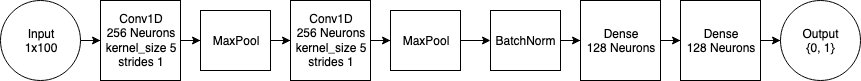
\includegraphics[width=\textwidth]{conv_architecture}
\centering
\end{figure}

\subsection{Fourier Convolutional Neural Network}
The Fourier Convolutional Neural Network leverages a custom "Fourier Layer", which moves the data into Fourier space via the Fast Fourier Transform before it performs a dot product on the input to the neuron.
Specifically, given an input $X^{(n)}$ and an output $A$, where the superscript is not an exponent, but instead indicates the layer of the input, the Fourier layer, $\ell$ acts on $X$: 
\begin{align*}
X^{(n+1)} & = a \\
& = \ell^{(n)}(X^{(n)}) \\
& = \sigma(\mathcal{F}^{-1}(\mathcal{F}(X^{(n)})\cdot \mathbf{W}^{(n)\top}))
\end{align*}

Where $\mathcal{F}$ is the Fast Fourier Transform, $\sigma$ is the activation function - ReLU in this case - and $\mathbf{W}$ is the weight matrix for layer n.

Our Fourier ``Convolutional'' neural network is a mirror image of our standard convolutional neural network, only with the convolutional layers replaced by Fourier layers.
Here, we put the word convolutional in scare quotes due to the fact that no actual convolution is performed and thus it is a misnomer.
To be more intellectually honest, we should refer to this network instead as a ``Fourier Transform Inner Product Network'', though this may confuse readers unfamiliar with the relationship.
In the interest of broad understanding, the term convolutional neural network is used when it helps elucidate meaning even in spite of being a slight misnomer.

\subsection{Wavelet Convolutional Neural Network} \label{wavelet cnn}
The Wavelet Convolutional Neural Network implements similar functionality to our Fourier Neural Network, using the Continuous Wavelet Transform in lieu of the Fourier transform.
Due to the fact that there is a time component and a frequency component, the wavelet neural network has a higher dimensionality than our other models. 

Details of the Wavelet Neural Network are pending a significant code revision.
This revision is due to some late work associated with the inversion of the continuous wavelet transform.

\subsection{Other Models} \label{other models}
Two baseline models were considered.
The first is the random forest model provided in the Scikit-learn library with no hyperparameter tuning.
Decision tree models are generally good at classification tasks~\cite{hastie01statisticallearning} but are weak classifiers which are sensitive to variance.
Random forests are a the result of averaging a large collection of de-correlated trees and provide a good benchmark as a na\"ive model - in the respect that it is untuned - for classification.

The other benchmark model is a Support Vector Classifier, again provided by the Scikit-learn library.
The rationale for using a Support Vector Machine is that we wanted to see if some hyperplane could be learned which would separate the data.
This model was again, na\"ive in the respect that it was merely the ``out of the box'' model, and so the classifier was built on top of the radial basis function kernel.
%\printbibliography[title={References}]
%\end{refsection}
%
%\begin{refsection}[myrefs.bib]
\chapter{\lipsum*[19][1]}
\label{chap:three}

% Introduction
\sect{\lipsum*[20][1]}

\subsect{\lipsum*[20][2]}

\lipsum[1-3]

\subsect{\lipsum*[20][3]}

\lipsum[4-5]

\subsect{\lipsum*[20][4]}

\lipsum[7-8]

\subsect{\lipsum*[20][5]}

\lipsum[10-12]

% Figure 3-1
\begin{figure}[tb]
   \centering
%   
\includegraphics[width=\textwidth,height=\textheight,keepaspectratio]{fig_3-1}
   
\includegraphics[scale=1]{fig_3-1}
   \caption[{\lipsum*[31][1]}]{\lipsum*[31][1-5]}
   \label{fig:fig_3-1}
\end{figure}

% Materials and Methods
\sect{\lipsum*[21][1]}

\subsect{\lipsum*[21][2]}

\lipsum[13]

\subsect{\lipsum*[21][3]}

\lipsum[14-15]

\subsect{\lipsum*[21][4]}

\lipsum[16-17]

\subsect{\lipsum*[21][5]}

\lipsum[18]

\subsect{\lipsum*[21][6]}

\lipsum[19-20]

\subsect{\lipsum*[21][7]}

\lipsum[21]

\subsect{\lipsum*[21][8]}

\lipsum[22]

\subsect{\lipsum*[21][9]}

\lipsum[23-24]

\subsect{\lipsum*[21][10]}

\lipsum[25-26]

\subsect{\lipsum*[21][11]}

\lipsum[27-28]

\subsect{\lipsum*[21][12]}

\lipsum[29-30]

\subsect{\lipsum*[21][13]}

\lipsum[31]

% Results
\sect{\lipsum*[22][1]}

\subsect{\lipsum*[22][2]}

\lipsum[27-32]

% Figure 3-2
\begin{figure}[p]
   \centering
%   
\includegraphics[width=\textwidth,height=\textheight,keepaspectratio]{fig_3-2}
   
\includegraphics[scale=1]{fig_3-2}
   \caption[{\lipsum*[32][1]}]{\lipsum*[32][1-5]}
   \label{fig:fig_3-2}
\end{figure}

\subsect{\lipsum*[22][3]}

\lipsum[33-35]

% Figure 3-3
\begin{figure}[p]
   \centering
%   
\includegraphics[width=\textwidth,height=\textheight,keepaspectratio]{fig_3-3}
   
\includegraphics[scale=1]{fig_3-3}
   \caption[{\lipsum*[33][1]}]{\lipsum*[33][1-5]}
   \label{fig:fig_3-3}
\end{figure}

\subsect{\lipsum*[22][4]}

\lipsum[36-37]

% Figure 3-4
\begin{SCfigure}[\sidecaptionrelwidth][p]
   \centering
%   
\includegraphics[width=\textwidth,height=\textheight,keepaspectratio]{fig_3-4}
   
\includegraphics[scale=0.90]{fig_3-4}
   \caption[{\lipsum*[34][1]}]{\lipsum*[34][1-5]}
   \label{fig:fig_3-4}
\end{SCfigure}

\subsect{\lipsum*[22][5]}

\lipsum[38-40]

% Figure 3-5
\begin{figure}[p]
   \centering
%   
\includegraphics[width=\textwidth,height=\textheight,keepaspectratio]{fig_3-5}
   
\includegraphics[scale=1]{fig_3-5}
   \caption[{\lipsum*[35][1]}]{\lipsum*[35][1-5]}
   \label{fig:fig_3-5}
\end{figure}

\subsect{\lipsum*[22][6]}

\lipsum[41-43]

% Figure 3-6
\begin{figure}[p]
   \centering
%   
\includegraphics[width=\textwidth,height=\textheight,keepaspectratio]{fig_3-6}
   
\includegraphics[scale=1]{fig_3-6}
   \caption[{\lipsum*[36][1]}]{\lipsum*[36][1-2]}
   \label{fig:fig_3-6}
\end{figure}

% Discussion
\sect{\lipsum*[22][7]}

\lipsum[44-51]

% Figure 3-7
\begin{figure}[p]
   \centering
%   
\includegraphics[width=\textwidth,height=\textheight,keepaspectratio]{fig_3-7}
   
\includegraphics[scale=1]{fig_3-7}
   \caption[{\lipsum*[37][1]}]{\lipsum*[37][1-2]}
   \label{fig:fig_3-7}
\end{figure}

% Figure 3-8
\begin{figure}[p]
   \centering
%   
\includegraphics[width=\textwidth,height=\textheight,keepaspectratio]{fig_3-8}
   
\includegraphics[scale=1]{fig_3-8}
   \caption[{\lipsum*[38][1]}]{\lipsum*[38][1-2]}
   \label{fig:fig_3-8}
\end{figure}

% Figure 3-9
\begin{figure}[p]
   \centering
%   
\includegraphics[width=\textwidth,height=\textheight,keepaspectratio]{fig_3-9}
   
\includegraphics[scale=1]{fig_3-9}
   \caption[{\lipsum*[39][1]}]{\lipsum*[39][1-2]}
   \label{fig:fig_3-9}
\end{figure}

% Figure 3-10
\begin{figure}[p]
   \centering
%   
\includegraphics[width=\textwidth,height=\textheight,keepaspectratio]{fig_3-10}
   
\includegraphics[scale=1]{fig_3-10}
   \caption[{\lipsum*[40][1]}]{\lipsum*[40][1-2]}
   \label{fig:fig_3-10}
\end{figure}

%\printbibliography[title={References}]
%\end{refsection}
%
%\begin{refsection}[myrefs.bib]
\chapter{\lipsum*[29][1]}
\label{chap:four}
%\newpage

% Introduction
\sect{\lipsum*[30][1]}

\subsect{\lipsum*[30][2]}

\lipsum[1-5]

\subsect{\lipsum*[30][3]}

\lipsum[6-7]

\subsect{\lipsum*[30][4]}

\lipsum[9-10]

 Figure 4-1
\begin{figure}[tb]
   \centering
%   
\includegraphics[width=\textwidth,height=\textheight,keepaspectratio]{fig_4-1}
   
\includegraphics[scale=1]{fig_4-1}
   \caption[{\lipsum*[41][1]}]{\lipsum*[41][1-5]}
   \label{fig:fig_4-1}
\end{figure}

% Materials and Methods
\sect{\lipsum*[31][1]}

\subsect{\lipsum*[31][2]}

\lipsum[11]

\subsect{\lipsum*[31][3]}

\lipsum[12-13]

\subsect{\lipsum*[31][4]}

\lipsum[14]

\subsect{\lipsum*[31][5]}

\lipsum[15]

\subsect{\lipsum*[31][6]}

\lipsum[16-17]

\subsect{\lipsum*[31][7]}

\lipsum[18]

\subsect{\lipsum*[31][8]}

\lipsum[20-21]

\subsect{\lipsum*[31][9]}

\lipsum[22]

\subsect{\lipsum*[31][10]}

\lipsum[25-26]

\subsect{\lipsum*[31][11]}

\lipsum[29-30]

\subsect{\lipsum*[31][12]}

\lipsum[31]

\subsect{\lipsum*[31][13]}

\lipsum[32]

\subsect{\lipsum*[31][14]}

\lipsum[33]

% Results
\sect{\lipsum*[32][1]}

\subsect{\lipsum*[32][2]}

\lipsum[34-35]

% Figure 4-2
\begin{figure}[p]
   \centering
%   
\includegraphics[width=\textwidth,height=\textheight,keepaspectratio]{fig_4-2}
   
\includegraphics[scale=0.90]{fig_4-2}
   \caption[{\lipsum*[42][1]}]{\lipsum*[42][1-5]}
   \label{fig:fig_4-2}
\end{figure}

\subsect{\lipsum*[32][3]}

\lipsum[36-37]

% Figure 4-3
\begin{figure}[p]
   \centering
%   
\includegraphics[width=\textwidth,height=\textheight,keepaspectratio]{fig_4-3}
   
\includegraphics[scale=1]{fig_4-3}
   \caption[{\lipsum*[43][1]}]{\lipsum*[43][1-5]}
   \label{fig:fig_4-3}
\end{figure}

\lipsum[45-49]

% Figure 4-4
\begin{figure}[p]
   \centering
%   
\includegraphics[width=\textwidth,height=\textheight,keepaspectratio]{fig_4-4}
   
\includegraphics[scale=1]{fig_4-4}
   \caption[{\lipsum*[44][1]}]{\lipsum*[44][1-5]}
   \label{fig:fig_4-4}
\end{figure}

\subsect{\lipsum*[32][4]}

\lipsum[51-52]

% Figure 4-5
\begin{figure}[p]
   \centering
%   
\includegraphics[width=\textwidth,height=\textheight,keepaspectratio]{fig_4-5}
   
\includegraphics[scale=0.95]{fig_4-5}
   \caption[{\lipsum*[45][1]}]{\lipsum*[45][1-5]}
   \label{fig:fig_4-5}
\end{figure}

\subsect{\lipsum*[32][5]}

\lipsum[56-59]

% Discussion
\sect{\lipsum*[33][2]}

\lipsum[61-65]


% Figure 4-6
\begin{figure}[p]
   \centering
%   
\includegraphics[width=\textwidth,height=\textheight,keepaspectratio]{fig_4-6}
   
\includegraphics[scale=0.95]{fig_4-6}
   \caption[{\lipsum*[46][1]}]{\lipsum*[46][1-5]}
   \label{fig:fig_4-6}
\end{figure}

% Figure 4-7
\begin{figure}[p]
   \centering
%   
\includegraphics[width=\textwidth,height=\textheight,keepaspectratio]{fig_4-7}
   
\includegraphics[scale=0.95]{fig_4-7}
   \caption[{\lipsum*[47][1]}]{\lipsum*[47][1-5]}
   \label{fig:fig_4-7}
\end{figure}

% Figure 4-8
\begin{figure}[p]
   \centering
%   
\includegraphics[width=\textwidth,height=\textheight,keepaspectratio]{fig_4-8}
   
\includegraphics[scale=1]{fig_4-8}
   \caption[{\lipsum*[48][1]}]{\lipsum*[48][1-5]}
   \label{fig:fig_4-8}
\end{figure}
%\printbibliography[title={References}]
%\end{refsection}
%
%\begin{refsection}[myrefs.bib]
\chap{Conclusions and general discussion}
\label{chap:conclusion}

\lipsum[1-12]

%\printbibliography[title={References}]
%\end{refsection}
%
%%%%% BACK MATTER %%%%%
%
%%% BIBLATEX BIBLIOGRAPHY %%%
%\footnotesize
\printbibliography[title={References},heading=bibintoc]
%
%%% BIBTEX BIBLIOGRAPHY %%%
%
% Use the IEEEtran.bst style file (bibtex)
%\bibliographystyle{IEEEtran}
%
% Name the bibliography
%\setbibref{References}
% Point to bibfile
%\footnotesize\bibliography{IEEEabrv,classics}
%\bibliography{IEEEabrv,classics}
%
% APPENDICES
\begin{appendices}
% Appendix I
%\thispagestyle{empty}
\footnotesize
% Setup and stylize appendices to integrate with TOC
\addtocontents{toc}{\protect\renewcommand\protect\cftchappresnum{\appendixname~}}
\renewcommand{\thechapter}{\Roman{chapter}}

% Stylize section header
\renewcommand{\thesection}{\Alph{section}.}

\begin{landscape}
% Appendix I: Oligonucleotide and probe sequences
%\addcontentsline{toc}{chapter}{Oligonucleotide and probe sequences}
\chapter{Oligonucleotide and probe sequences}
\label{append:one}
%
\begin{longtable}{p{0.15in}p{1.25in}>{\itshape}p{2.25in}>{\ttfamily}p{4.10in}}
% header ------------------------
\caption{Oligonucleotide and probe sequences}\\
\toprule
\multicolumn{1}{l}{\textnumero}&
\multicolumn{1}{l}{Name}&
\multicolumn{1}{l}{Note}&
\multicolumn{1}{l}{Sequence}\\
\midrule
\endfirsthead
\caption{Oligonucleotide and probe sequences}\\
\toprule
\multicolumn{1}{l}{\textnumero}&
\multicolumn{1}{l}{Name}&
\multicolumn{1}{l}{Note}&
\multicolumn{1}{l}{Sequence}\\
\midrule
\endhead
\\

% Inelegant header
&\multicolumn{3}{c}{\large\textbf{General}}\\[1em]
%
1 & SP6-F &
SP6 Promoter Primer &
\seqsplit{GATTTAGGTGACACTATAG}\\
%
2 & T7-F &
T7 Promoter Primer &
\seqsplit{TAATACGACTCACTATAGG}\\[1em]
%
% Inelegant header
&\multicolumn{3}{c}{\large\textbf{qPCR oligos \& probes}}\\[1em]
%
3 & EGFP-615F &&
\seqsplit{GTCCGCCCTGAGCAAAGA}\\
%
4 & EGFP-668R &&
\seqsplit{TCCAGCAGGACCATGTGATC}\\
%
5 & EGFP-634T &
EGFP probe &
\seqsplit{CCCAACGAGAAGCG}\\
%
\bottomrule
\end{longtable}
\end{landscape}


% Appendix II
\chapter{Another Appendix}
\label{append:two}


\end{appendices}
%
%%% CV %%%
% Add to TOC
\addcontentsline{toc}{chapter}{Curriculum vitae}

% If you want to remove page numbers
%\pagestyle{empty}


% Default settings for enumerate environment
\setenumerate{wide=0em,%
              leftmargin=*,
              labelindent=0pt,
              label=\textbullet,
              noitemsep,
              topsep=0pt,
              parsep=0pt,
              before=\rmfamily}

% Remove indentation
\setlength{\parindent}{0pt}

% Space between paragraphs
\setlength{\parskip}{6pt}

% No added spaces after periods
\frenchspacing

% For a reasonable fit
\footnotesize

\textbf{\small Curriculum Vitae\hfill\large Erick Galinkin\hfill\small June, 2020}
\begin{center}
(+1) 631.830.7524\\
{\color{blue} \ul{\sffamily\textit{egalink1@jhu.edu}}}
\end{center}

% change font 
\sffamily

\textbf{EDUCATION AND DEGREES}

\ul{2018--Present} Graduate student,
Department of Applied and Computational Mathematics\\
Johns Hopkins University

\ul{20XX--20XX} Undergraduate student,
Department of Biology
University of California


\textbf{RESEARCH EXPERIENCE}

\textit{Johns Hopkins University, Some specific school}\\
\textit{Department of Biology\hfill(MONTH YEAR-Present)}\\
\textbf{\rmfamily Graduate Student in the laboratory of a \ul{Principal Investigator}}

\begin{enumerate}
\item Some thing I did.
\item Another thing I did.
\item Yet another thing I did.
\end{enumerate}

\textit{A previous academic research institution, LOCATION\hfill(MONTH YEAR-MONTH YEAR)}\\
\textbf{\rmfamily Post-baccalaureate Researcher in the laboratory of a \ul{Principal Investigator}}

\begin{enumerate}
\item A thing I did.
\item Another thing I did.
\end{enumerate}

\textit{A previous academic research institution, LOCATION\hfill(MONTH YEAR-MONTH YEAR)}\\
\textbf{\rmfamily A previous position in the laboratory of a \ul{Principal Investigator}}

\begin{enumerate}
\item Some thing I did.
\item Another thing I did.
\item Yet another thing I did.
\end{enumerate}

\textbf{TECHNIQUES AND SKILLS}

\textbf{\rmfamily Molecular Techniques}

\textrm{\noindent DNA/RNA/Protein extraction and purification ; PCR ; RT-PCR ; Quantitative 
PCR ; DNA Sequence Analysis ; Southern Blot ; Western Blot ; SDS-PAGE ; Ultra-Centrifugation 
; Agarose Gel Electrophoresis/Imaging ; \textit{Drosophila} Microinjection ;\textit{ 
Anopheles} Microinjection ; Fluorescence Microscopy ; Immunofluorescence Microscopy ; 
Cell/tissue Culture ; Cell Transfection ; Antiseptic Technique}

\textbf{\rmfamily Computing and Other Skills}
\begin{enumerate}
\item Power user of both Windows and Macintosh platform software and hardware
\item Basic user of Linux/Unix systems
\item Basic Perl programming
\item Basic R programming
\item Proper waste disposal practices and safety training
\item Radioactive isotope certification and safety training
\item Ethical use of vertebrate animals (mice) in research training
\end{enumerate}

\textbf{TEACHING EXPERIENCE}

\textit{Johns Hopkins University, Some school\hfill(MONTH YEAR-MONTH YEAR)}\\
\textbf{\rmfamily Teaching Assistant}
\begin{enumerate}
\item Graduate Student Instructor for a class
\end{enumerate}

\textit{University of California\hfill(MONTH YEAR-MONTH YEAR)}\\
\textbf{\rmfamily Teaching Assistant}
\begin{enumerate}
\item Undergraduate Student Instructor for a class.
\end{enumerate}


\textbf{PUBLICATIONS}

% change font back to roman
\rmfamily

{\color{blue} \ul{The title of my article.}} 
A. Anderson, \textbf{Myself}, B. Baldwin, C. Cortez and 
D. Dylan. \textit{Journal Name} \textbf{VOLUME}. PAGES (YEAR).

{\color{blue} \ul{The title of my article.}} 
A. Anderson, \textbf{Myself}, B. Baldwin, C. Cortez and 
D. Dylan. \textit{Journal Name} \textbf{VOLUME}. PAGES (YEAR).

{\color{blue} \ul{The title of my article.}} 
A. Anderson, \textbf{Myself}, B. Baldwin, C. Cortez and 
D. Dylan. \textit{Journal Name} \textbf{VOLUME}. PAGES (YEAR).

{\color{blue} \ul{The title of my article.}} 
A. Anderson, \textbf{Myself}, B. Baldwin, C. Cortez and 
D. Dylan. \textit{Journal Name} \textbf{VOLUME}. PAGES (YEAR).

{\color{blue} \ul{The title of my article.}} 
A. Anderson, \textbf{Myself}, B. Baldwin, C. Cortez and 
D. Dylan. \textit{Journal Name} \textbf{VOLUME}. PAGES (YEAR).

%
%%% Biographical Sketch %%%
\chap{Biographical sketch}
% Reset the default paragraph style
\normalsize
\nonfrenchspacing
\doublespacing
\setlength{\parindent}{15pt} % default value for 12pt report
\setlength{\parskip}{3pt} % document default

% BIOSKETCH TEXT HERE
Erick Galinkin was born in Port Jefferson, New York.
After graduating from Miller Place High School in 2007, he spent a brief time at Stony Brook University where he studied Chemistry. 
In 2008, he joined the United States Air Force as a Chinese Language Analyst and spent 6 years enlisted, separating as a Staff Sergeant.
During his time in the Air Force, Erick obtained an Associate's Degree in Mandarin Chinese from the Defense Language Institute and a Bachelor's Degree in Cybersecurity from the University of Maryland Global Campus.
In 2014, Erick began working as a Research Engineer for Cisco Systems and shortly thereafter began pursuing a masters in information assurance, also from University of Maryland Global Campus, graduating in 2017.
Erick has also obtained a graduate certificate in bioinformatics from UMGC, and worked as a Senior DevOps Engineer at Optiv prior to starting at Johns Hopkins.
Beginning in September 2018, Erick enrolled at Johns Hopkins while working as a Security Research Scientist at Netskope. 
In January, 2020 he began work as a Principal AI Researcher at Rapid7.
Presently, Erick has accepted an offer to further his studies as a PhD student in Computer Science at Drexel University.
%
\end{document}